\chapter{Opportunities and internals of SUDS}

\section{Introduction}

As I described in section \ref{suds}, SUDS is the de facto way of consuming web services in Python. One of the most compelling features lies within its simplicity and user friendliness. These help in the beginning, by making it really easy to create a working prototype in no time, both by using the interactive shell and writing scripts -- but later, the code is still readable, and at the same time, caching helps eliminating the performance trade-off. A sample run, consuming a currency rate service using SUDS in the interactive Python shell can be seen in Figure \ref{fig:suds-currency}.

\begin{figure}[htbp]
 \centering
\begin{lstlisting}[numbers=off, basicstyle=\footnotesize\ttfamily]
Python 2.7.2+ (default, Aug 16 2011, 07:03:08)
[GCC 4.6.1] on linux2
Type "help", "copyright", "credits" or "license" for more information.
>>> from suds.client import Client
>>> url = 'http://www.webservicex.net/CurrencyConvertor.asmx?WSDL'
>>> c = Client(url)
>>> print c

Suds ( https://fedorahosted.org/suds/ )  version: 0.4.1 (beta)  build: R703-20101015

Service ( CurrencyConvertor ) tns="http://www.webserviceX.NET/"
   Prefixes (1)
      ns0 = "http://www.webserviceX.NET/"
   Ports (2):
      (CurrencyConvertorSoap)
         Methods (1):
            ConversionRate(Currency FromCurrency, Currency ToCurrency, )
         Types (1):
            Currency
      (CurrencyConvertorSoap12)
         Methods (1):
            ConversionRate(Currency FromCurrency, Currency ToCurrency, )
         Types (1):
            Currency


>>> c.service.ConversionRate('EUR', 'HUF')
315.6003
\end{lstlisting}
 \caption{Requesting currency conversion rate using SUDS}
 \label{fig:suds-currency}
\end{figure}

\section{Internal structure}

In order to improve SUDS, I had to discover its inner workings -- the documentation covered standard use-cases pretty well, but told little about architecture. I split the code in time domain into two pieces, the separator being the end of \emph{suds.client.Client} object instantiation Before that, WSDL fetching and parsing happens, and afterwards, during invocations, SOAP messages are built, sent, and responses are parsed and returned.

\subsection{Client proxy instantiation}

The \emph{Client} object is the ``soul'' of the library and can be found in the \emph{suds.client} module. The constructor has one fixed parameter (the WSDL URL), all the others get stored in a dictionary for later use. Upon creation, the WSDL gets fetched and all the plugins (see section \ref{sudsPlugins}) are notified. The WSDL is parsed for service definitions and schemas -- these are used to create the factories later used for the instantiation of complex objects, and for lookup on method invocation. The root element of the DOM representing the WSDL is stored for the whole lifecycle of the object in the \emph{wsdl} attribute, and the \emph{services} attribute is set to an instance of \emph{ServiceSelector}, the key to method invocation (see section \ref{sudsInvocation}).

\subsection{Instantiation of complex objects}

Since many web services expect complex objects as an input parameter, its instantiation is a problem present in all web services clients. As I mentioned in section \ref{ZSI}, ZSI solved this problem in the ``classic'' way, with source code generation, which makes experimentation tedious and increases turnaround times. In contrast, SUDS offers a solution implementing the Factory pattern, a ``method'' (actually a callable attribute) of the \emph{Client} class, which returns an appropriate object, given a class name. This object can be later populated as a regular object, or its attributes can be used in case of enumerations. Since version 0.3.8, SUDS also supports the implicit conversion of native Python dictionary objects to SOAP complex types, using the keys as attribute names, which can lead to cleaner code in some cases.

\subsection{Service method invocation}
\label{sudsInvocation}

As it can be seen on Figure \ref{fig:suds-currency}, users simply reference method names, like it's the attribute of the service object -- behind the scenes, the \emph{services} attribute makes use of Python dynamic dispatch. In this case, the \emph{suds.client.ServiceSelector} class overrides the special \verb|__getattr__| method, thus the sample invocation on Figure \ref{fig:suds-currency} caused the Python runtime to first call \verb|c.service.__getattr__| with \emph{getConversionRate} as a string parameter. In case of success, the method returns a callable (function pointers in C/C++, delegates in C\#), which is invoked next with the actual parameters supplied by the user to the \emph{getConversionRate} method call. This makes use of another Python feature -- the positional and named parameters can be retrieved as a list and dictionary, respectively.

If multiple ports and/or services are available, the same dynamic dispatch is played again (sometimes with \verb|__getitem__| instead of \verb|__getattr__|, the complete lookup chain is \emph{Client} $\rightarrow$ \emph{ServiceSelector} $\rightarrow$ \emph{PortSelector} $\rightarrow$ \emph{MethodSelector} $\rightarrow$ \emph{Client}. The second and third step can be implicit, in that case, the first service or port will be used -- in the end, the program flow enters \emph{Client} at the \emph{invoke} method, with completely specified parameters. The parameters are transformed into the SAX representation of a SOAP envelope, as it can be seen on Figure \ref{fig:sudsMessage}, which in turn can be serialized as an XML string. This binary data is now sent using the transport layer (currently \emph{urllib2}), which returns the response -- the same process gets repeated, as with the request, but reversed. In the end, the caller receives the response transformed back to instances of data types native to Python.

\begin{figure}[htbp]
 \centering
 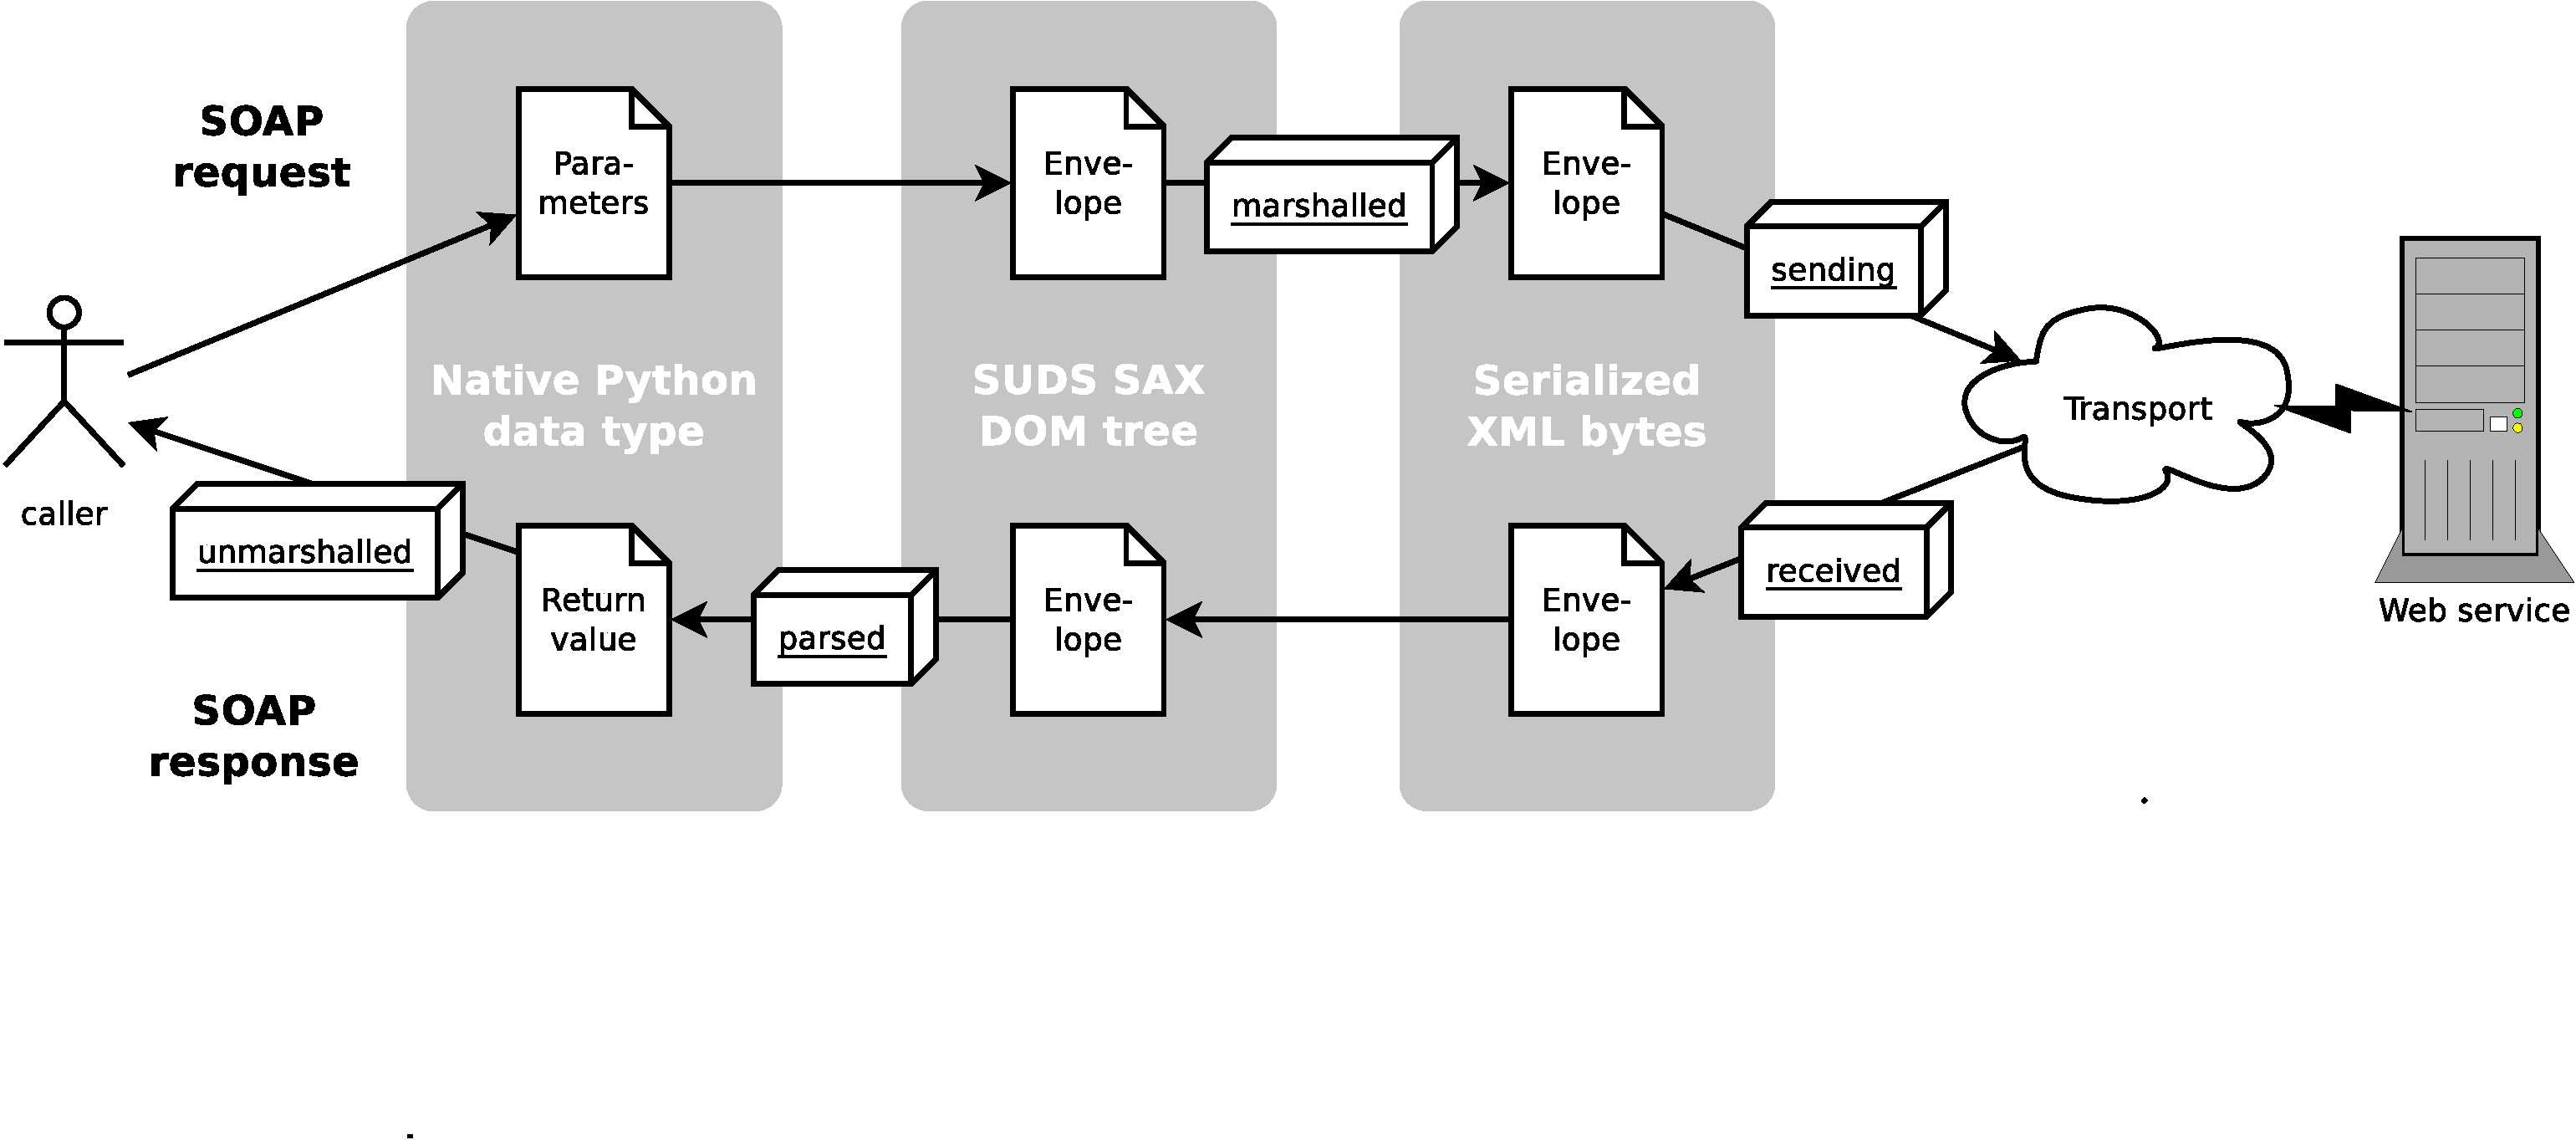
\includegraphics[width=\textwidth]{images/sudsMessage.pdf}
 \caption{SUDS message processing}
 \label{fig:sudsMessage}
\end{figure}

\subsection{Document Object Model of SUDS}

As \cite{w3schools-domintro} defines it, ``XML DOM is a standard for how to get, change, add, or delete XML elements'', which is the better way to construct XML output -- the worse being string concatenation. SUDS has its own implementation, and as \cite{suds-doc} states, it ``was written [because] elementtree and other [Python] XML packages either: have a DOM API which is very unfriendly or: (in the case of elementtree) do not deal with namespaces and especially prefixes sufficiently'' -- and in retrospect, it was a perfectly sane decision back then. The SUDS DOM resides in the \emph{suds.sax} module, and interfaces the outside world with the Python built-in SAX parser. It registers itself as a SAX event handler, and builds the document tree from its own objects in response to parsing events, so there is a clear separation between the Python XML library and the implementation of SUDS.

Although now we have LXML (see section \ref{lxml}) which would have satisfied those conditions (and is used by rpclib), it was probably not in this state of maturity, when the SUDS project kicked off. It has its own peculiarities, such as namespace handling is done using (prefix, namespace) tuples -- in contrast with standard notations such as dictionary objects or James Clark style. This self-developed solution also caused the appearance of ``double namespaces'' -- the SOAP-ENV namespace was declared with one prefix for the envelope and header, and another for the body. While working on improving SUDS, I also found that it had several deficiencies, for instance, there's no way of handling attributes with namespaces. It could seem, that now it'd be time to replace the library with a thin wrapper around LXML or some other functionally equivalent components, but it'd break existing code depending on the internals of SUDS.

\section{Opportunities}

\subsection{Current WS-Security implementation}

Using the examples in the SUDS documentation, it was easy to find, that the WSSE implementation had a clean OO design, as it can be seen on Figure \ref{fig:clsdSudsWsse}. The \emph{Security} object encapsulated the collection of tokens as a smart container. During invocation, the \emph{xml} method gets called, and it simply constructs an appropriate \emph{wsse:Security} header, and fills it with the result of the \emph{xml} methods of all the tokens, before returning it to the caller.

The class diagram also makes it clear, that there is no support for digital signatures or encryption -- although surprisingly, there are (currently unused) namespaces defined in the source code for both of them.

\begin{figure}[htbp]
 \centering
 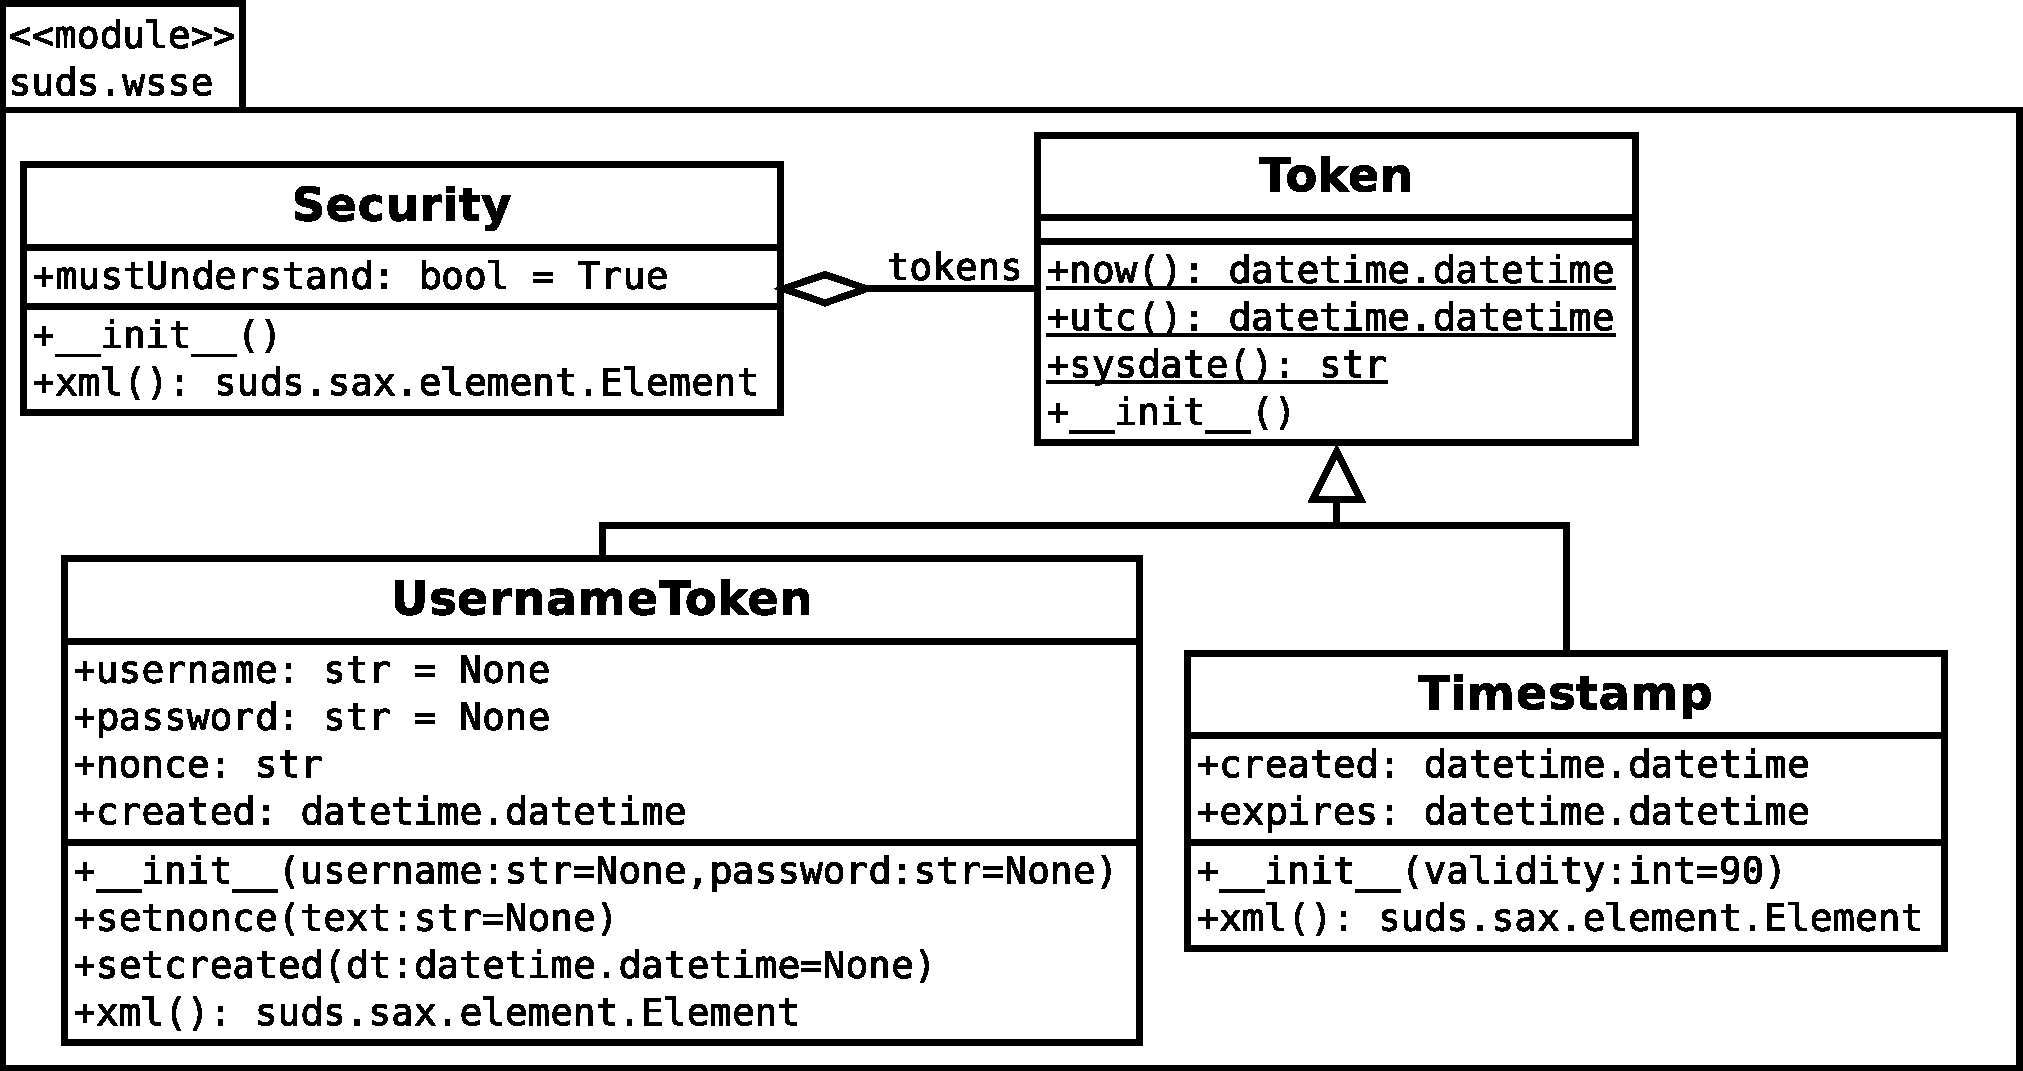
\includegraphics[width=12cm]{images/clsdSudsWsse.pdf}
 \caption{Class diagram of the \emph{suds.wsse} module}
 \label{fig:clsdSudsWsse}
\end{figure}

\subsubsection{Timestamp}

As \cite{ibm-timestamp} and \cite{msdn-wss} agree, WS\hyp{}Security timestamp is useful in case the freshness of the message needs to be verified -- this can be important to avoid replay attacks, or to resolve issues with two or more messages causing contradiction. The standard itself is trivial to implement, and based on my observations of the codebase, the SUDS solution is complete and correct -- I later verified it also by connecting it to a properly set up CXF service. The \emph{suds.wsse.Timestamp} class even helps the user by automatically setting and formatting the creation and expiration time -- although the lack of digital signature implementation makes this feature unusable for security purposes.

\subsubsection{UsernameToken}
\label{sudsUsernameToken}

According to \cite{suds-doc}, SUDS had a UsernameToken implementation, so I tried it with an Apache CXF service. As it turned out, the burden of digest creation was put on the caller, and the type of the password wasn't specified in the token, as required by WS\hyp{}Security. This limits the usability of the solution, but it's certainly easier to extend it, than creating a new implementation from scratch.

\subsection{Plugin system}
\label{sudsPlugins}

Since version 0.4, SUDS has a plugin system, that allows developers to extend its functionality without the need to maintain a separate version of the library. During the construction of a \emph{Client} object, a list of plugin instances can be supplied, and their methods will be called at specific points of the SUDS lifecycle. Most useful use-cases include inspection and (optional) modification of the internal status. These objects should inherit one of the classes in the \emph{suds.plugin} module, and this way, only methods of interest need overriding -- those (currently three) ancestors define the points of interaction available.

The full list of these can be found in \cite{suds-doc}, I'd emphasize the one, I found good use of; it's called \emph{MessagePlugin}, has five possible points of interaction, and thus allows for a fine-grained control over the SOAP message. As it can be seen on Figure \ref{fig:sudsMessage}, interception and modification is possible at all important places, with the data available in the current format (SUDS objects, DOM tree, or bytes) using holder objects called \emph{context}. One surprising thing I found was, that if plugin execution raises an exception, instead of the call failing, processing continues, and the details get logged using the Python logging system -- which means silent fail by default. Still, I found the plugin system to be a well-designed, usable form of extending SUDS.
